\chapter{Cox proportional hazards models}
\label{cha:cox}

\section{Introduction}
\label{sec:cox-introduction}
This chapter explains the cox proportional hazards model~\cite{simon2011regularization}\cite{tibshirani1997lasso}\cite{wikicox}. This is a model that is used in survival analysis. The first section explains what survival analysis means and how it is different from the generalized linear models. Next we will define what the proportional hazards assumption is and lastly we will show kaplan-meier survival curves and how we can compute them from hazard functions.

\section{Survival analysis}
\label{sec:cox-survival-analysis}
Survival analysis points to the fact that the outcome variables are time-to-event datapoints. A common example in biomedical research would be the time between the start of a patients treatment and the time of death. Note however that not all patients have to die in order to be useful in a survival analysis. A second outcome variable is used to indicate whether the patient survived until the end of the study, or not. This (often binary) variable is called the censoring variable. \\ \\
A typical outcome in survival analysis is thus represented by two vectors: a time to event vector and a censoring vector. An example is shown in table \ref{tab:cox-example-outcome}.
\begin{table}
	\centering
	\begin{tabular}{cc}
		\toprule
		Time (days) & Censor\\
		\midrule
		249 & 1 \\
		345 & 1 \\
		152 & 1 \\
		452 & 0 \\
		120 & 1 \\
		... & ... \\
		\bottomrule
	\end{tabular}
	\caption{Example outcomes for survival data}
	\label{tab:cox-example-outcome}
\end{table}
The idea of survival analysis is now to find a pattern between a set of explanatory variables and the time-to-event. A common term used in survival analysis is hazard, meaning 'risk of the event occurring'. A resulting model from survival analysis usually contains two components. The first component is a $\lambda_{0}(t)$ baseline hazard function. This function describes how the risk of the event occurring changes with time, assuming there is no influence from any of the explanatory variables. The second component describes the influence of each explanatory variable on the hazard. This brings us to the notion of proportional hazards which is the topic of the next section.

\section{Cox proportional hazards model}
\label{sec:cox-proportional-hazards-model}
\subsection{Proportional hazards condition}
The proportional hazards condition means that we assume that hazard ratios are independent of time. A hazard ratio is the relative risk between two entities (patients). Furthermore the condition states that changes in the explanatory variables have an exponential effect on the hazard. The following paragraphs explain these statements in more detail.\\ \\
If we assume the proportional hazards condition to be true then this gives us the opportunity to estimate the effect of explanatory variables without dealing with the underlying baseline hazard function. This was an observation made by Sir David Cox~\cite{cox1972life}, hence the name of the model. We can represent the cox model as follows:
\begin{equation}
\begin{split}
\lambda_{i}(t) = \lambda_{0}(t)e^{X_{i1}\beta_{1} + ... + X_{iN}\beta_{N}}
\end{split}
\end{equation}
where
\begin{itemize}
	\item $\lambda_{i}(t)$ is the hazard for patient i at time t.
	\item $\lambda_{0}(t)$ is the baseline hazard at time t.
	\item $X_{i1} ... X_{iN}$ are the values of the explanatory variables for patient i.
	\item $\beta_{1} ... \beta_{N}$ are the values of the coefficients for each explanatory variable.
\end{itemize}
Now, let's look at relative risks between two patients:
\begin{equation}
\begin{split}
\frac{\lambda_{i}(t)}{\lambda_{j}(t)} 
= \frac{\lambda_{0}(t)e^{X_{i1}\beta_{1} + ... + X_{iN}\beta_{N}}}{\lambda_{0}(t)e^{X_{j1}\beta_{1} + ... + X_{jN}\beta_{N}}}
= e^{(X_{i1}-X_{j1})\beta_{1} + ... + (X_{iN}-X_{jN})\beta_{N}}
\end{split}
\end{equation}
This quantity is called the hazard ratio. Notice that this ratio does not depend on time. This means that if at the start of the study a patient has twice the risk of the event occurring compared to another patient, it will have twice the risk at any other time aswell. It's risk remains proportional, independent of time. \\ \\
We can also compute the effect on the hazard for a unit increase in an explanatory variable $X_{j}$. In the following formula the subscripts i that were used to indicate the patient have been omitted since this is patient independent. The hazard ratio then becomes:
\begin{equation}
\begin{split}
\frac{\lambda(t|X_{j}+1)}{\lambda(t|X_{j})} = e^{(X_{j}+1-X_{j})\beta_{j}} = e^{\beta_{j}}
\end{split}
\end{equation}
It is directly given by the exponential of the coefficient for the explanatory variable. This reflects the proportional hazards assumption that hazard ratios do not depend on time and that explanatory variables have an exponential effect on the hazard.
\subsection{Using the hazard ratio}
The proportional hazards assumption allows us to compute relative risks or hazard ratios without knowing the actual baseline hazard function. Knowing just relative ratios can be very useful however. Imagine the following scenario: we want to test if a certain drug increases the survivability of patients with a specific disease. We randomly give half of the patients the actual drug, the other half receives a placebo (or nothing at all). Performing a survival analysis using a cox model then allows us to compute the ratio of the hazards for the two groups. The coefficient for the explanatory variable that indicates which patients received the drug and which did not then tells us the effect of the drug on the hazard. We could then make a statement such as: "Taking the drug tends to half the risk of the event occurring (at any time)." This is obviously a useful result to support further research or development for the drug.

\subsection{Kaplan-Meier survival curves}
Kaplan-Meier survival curves~\cite{goel2010understanding} are often used in survival analysis. These curves show the probability of surviving up to any point t. It is thus a declining curve starting from 1 at $t=0$. An example curve is shown on figure \ref{fig:cox-example-kaplan-meier}.
\begin{figure}
	\centering
	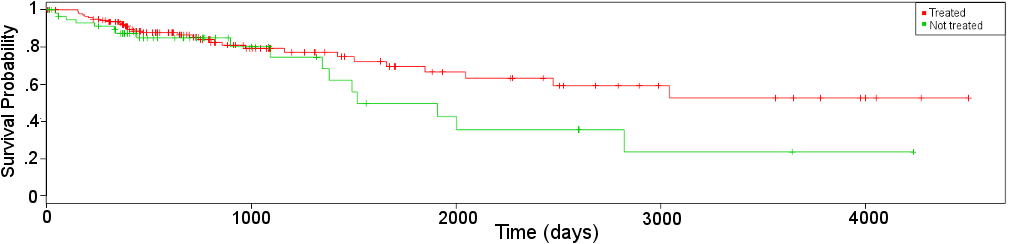
\includegraphics[scale=0.4]{images/example_kaplan_meier_curve}
	\caption{Example Kaplan-Meier survival curve. Red and green lines represent survival probabilities for treated and untreated patient-groups respectively.}
	\label{fig:cox-example-kaplan-meier}
\end{figure}
In formula notation we could write this as:
\begin{equation}
\begin{split}
S(t) = P(T > t)
\end{split}
\end{equation}
where
\begin{itemize}
	\item $S(t)$ is the survival function
	\item $P(x)$ means 'the probability of x'
	\item $T$ is the observed event time (e.g. death)
	\item $t$ is the time variable
\end{itemize}
\subsubsection{Linking hazard to survival}
Creating a kaplan-meier survival curve based on the outcome vectors (time and censoring) is very straightforward to do, it is simply a visual representation of the event occurring at certain times. However when we create a model that tries to explain these outcomes from explanatory variables we end up with a hazard function. In order to create survival curves we have to link this hazard function to the survival function~\cite{survivalmodels}. Recall the hazard function $\lambda(t)$ from section \ref{sec:cox-proportional-hazards-model}. We could write this function in a similar probabilistic notation as we did for the survival function:
\begin{equation}
\begin{split}
\lambda(t) = \lim\limits_{\delta\rightarrow0}\frac{P(t < T \leq t+\delta | T  > t)}{\delta}
\end{split}
\end{equation}
this is really just the definition of hazard: the risk of the event happening at time t is defined as the event happening during an infinitesimal timeframe after time t, given that the event has not happened yet up to time t. As we take the limit $\delta\rightarrow0$ this becomes an instantaneous hazard. We can now apply the conditional probability rule $P(A|B) = \frac{P(A \cap B)}{P(B)}$ to get:
\begin{equation}
\begin{split}
\label{eq:cox-hazard}
\lambda(t) &= \lim\limits_{\delta\rightarrow0}\frac{P(t < T \leq t+\delta \cap t < T)}{\delta}\frac{1}{P(T>t)} \\
&= \lim\limits_{\delta\rightarrow0}\frac{P(t < T \leq t+\delta)}{\delta}\frac{1}{S(t)} \\
&= \lim\limits_{\delta\rightarrow0}\frac{P(t < T) - P(t+\delta\leq T)}{\delta}\frac{1}{S(t)} \\
&= -\lim\limits_{\delta\rightarrow0}\frac{P(t+\delta\leq T) - P(t < T)}{\delta}\frac{1}{S(t)} \\
&= -\frac{\partial S(t)}{\partial t}\frac{1}{S(t)} \\
&= -\frac{S'(t)}{S(t)}
\end{split}
\end{equation}
Let's look at this result in an intuitive way. Assume the event we are talking about is dying. The hazard function then tells me what the risk is of dying at time $t$. Equation \ref{eq:cox-hazard} tells us that this is equal to $-\frac{S'(t)}{S(t)}$. There are three parts to explain here:
\begin{itemize}
	\item $\frac{1}{S(t)}$: The first thing we have to do is survive up to time $t$. Otherwise it makes no sense to ask what the risk of dying at time $t$ is. The survival function tells us how probable it is to survive up to time $t$ so dividing by this quantity exactly provides what we need. If $S(t)$ is large, then this means many people survive up to time $t$ and so the risk is low. If $S(t)$ is small then few people actually survive up to time $t$ and thus the risk of having to survive up to this point gets bigger.
	\item $S'(t)$: Now that we have survived up to time $t$, we need to calculate the risk of dying at this point in time. Remember that the survival curve declines whenever people die at certain points in time. The slope of this function therefore tells us how many people die at that time $t$. If $S'(t)$ is very large, it means that many people die here. The risk of dying thus becomes large.
	\item The hazard is supposed to be a positive quantity. Since the survival function is a strictly declining curve (people usually don't resurrect from the dead), $S'(t)$ is negative. Therefore we need the minus sign to end up with a positive result.
\end{itemize}
Next, using the chain rule, we can observe that
\begin{equation}
\begin{split}
\label{eq:cox-survival}
\frac{\partial log(S(t))}{\partial t} = \frac{S'(t)}{S(t)}
\end{split}
\end{equation}
and thus combining equations \ref{eq:cox-hazard} and \ref{eq:cox-survival}:
\begin{equation}
\begin{split}
\lambda(t) &= -\frac{\partial log(S(t))}{\partial t}
\end{split}
\end{equation}
\begin{equation}
\begin{split}
\label{eq:cox-int-hazard}
\int_{0}^{t}\lambda(t)dt &= \int_{0}^{t}-\frac{\partial log(S(t))}{\partial t}dt
\end{split}
\end{equation}
The left hand side of equation \ref{eq:cox-int-hazard} is called the cumulative hazard fuction and often denoted $\Lambda(t)$. We can then write:
\begin{equation}
\begin{split}
\Lambda(t) &= -log(S(t))
\end{split}
\end{equation}
\begin{equation}
\begin{split}
\label{eq:cox-survival-hazard-link}
S(t) &= e^{-\Lambda(t)}
\end{split}
\end{equation}
Equation \ref{eq:cox-survival-hazard-link} allows us to relate the survival function to the hazard function. This allows us to create survival curves for any form of hazard function. The only thing that is left to do is to define the baseline hazard function, because otherwise we could not compute the integral in $\Lambda(t)$ . Usually an estimator based on likelihood is used to estimate the baseline hazard function. There are many forms available for this estimator~\cite{royston2011estimating}, but we will not go into any more detail here.

\section{Conclusion}
\label{sec:cox-conclusion}
In this chapter we have explained the cox proportional hazards method. We have shown that it is used for survival analysis, where the targets are time and censoring variables. We have explained the proportional hazards assumption and shown its implications. Lastly we have shown how we can compute survival curves using the Kaplan-Meier method and we have shown a relationship between the hazard function and the survival function.
%%% Local Variables: 
%%% mode: latex
%%% TeX-master: "thesis"
%%% End: 
